%%%%%%%%%%%%%%%%%%%%%%%%%%%%%%%%%%%%%%%%%
% Programming/Coding Assignment
% LaTeX Template
%
% This template has been downloaded from:
% http://www.latextemplates.com
%
% Original author:
% Ted Pavlic (http://www.tedpavlic.com)
%
% Note:
% The \lipsum[#] commands throughout this template generate dummy text
% to fill the template out. These commands should all be removed when 
% writing assignment content.
%
% This template uses a Perl script as an example snippet of code, most other
% languages are also usable. Configure them in the "CODE INCLUSION 
% CONFIGURATION" section.
%
%%%%%%%%%%%%%%%%%%%%%%%%%%%%%%%%%%%%%%%%%

%----------------------------------------------------------------------------------------
%	PACKAGES AND OTHER DOCUMENT CONFIGURATIONS
%----------------------------------------------------------------------------------------

\documentclass{article}

\usepackage{fancyhdr} % Required for custom headers
\usepackage{lastpage} % Required to determine the last page for the footer
\usepackage{extramarks} % Required for headers and footers
\usepackage[usenames,dvipsnames]{color} % Required for custom colors
\usepackage{graphicx} % Required to insert images
\usepackage{listings} % Required for insertion of code
\usepackage{courier} % Required for the courier font
\usepackage{lipsum} % Used for inserting dummy 'Lorem ipsum' text into the template

% Margins
\topmargin=-0.45in
\evensidemargin=0in
\oddsidemargin=0in
\textwidth=6.5in
\textheight=9.0in
\headsep=0.25in

\linespread{1.1} % Line spacing

% Set up the header and footer
\pagestyle{fancy}
\lhead{\hmwkAuthorName} % Top left header
\chead{} % Top center head
\rhead{\hmwkClass \firstxmark} % Top right header
\lfoot{\lastxmark} % Bottom left footer
\cfoot{} % Bottom center footer
\rfoot{Page\ \thepage\ of\ \protect\pageref{LastPage}} % Bottom right footer
\renewcommand\headrulewidth{0.4pt} % Size of the header rule
\renewcommand\footrulewidth{0.4pt} % Size of the footer rule

\setlength\parindent{0pt} % Removes all indentation from paragraphs

%----------------------------------------------------------------------------------------
%	CODE INCLUSION CONFIGURATION
%----------------------------------------------------------------------------------------

\definecolor{MyDarkGreen}{rgb}{0.0,0.4,0.0} % This is the color used for comments
\lstloadlanguages{Python} % Load Perl syntax for listings, for a list of other languages supported see: ftp://ftp.tex.ac.uk/tex-archive/macros/latex/contrib/listings/listings.pdf
\lstset{language=Python, % Use Perl in this example
        frame=single, % Single frame around code
        basicstyle=\small\ttfamily, % Use small true type font
        keywordstyle=[1]\color{Blue}\bf, % Perl functions bold and blue
        keywordstyle=[2]\color{Purple}, % Perl function arguments purple
        keywordstyle=[3]\color{Blue}\underbar, % Custom functions underlined and blue
        identifierstyle=, % Nothing special about identifiers                                         
        commentstyle=\usefont{T1}{pcr}{m}{sl}\color{MyDarkGreen}\small, % Comments small dark green courier font
        stringstyle=\color{Purple}, % Strings are purple
        showstringspaces=false, % Don't put marks in string spaces
        tabsize=5, % 5 spaces per tab
        %
        % Put standard Perl functions not included in the default language here
        morekeywords={rand},
        %
        % Put Perl function parameters here
        morekeywords=[2]{on, off, interp},
        %
        % Put user defined functions here
        morekeywords=[3]{test},
       	%
        morecomment=[l][\color{Blue}]{...}, % Line continuation (...) like blue comment
        numbers=left, % Line numbers on left
        firstnumber=1, % Line numbers start with line 1
        numberstyle=\tiny\color{Blue}, % Line numbers are blue and small
        stepnumber=5 % Line numbers go in steps of 5
}

% Creates a new command to include a perl script, the first parameter is the filename of the script (without .pl), the second parameter is the caption
\newcommand{\pythonscript}[2]{
\begin{itemize}
\item[]\lstinputlisting[caption=#2,label=#1]{#1.py}
\end{itemize}
}

%----------------------------------------------------------------------------------------
%	DOCUMENT STRUCTURE COMMANDS
%	Skip this unless you know what you're doing
%----------------------------------------------------------------------------------------

% Header and footer for when a page split occurs within a problem environment
\newcommand{\enterProblemHeader}[1]{
\nobreak\extramarks{#1}{#1 continued on next page\ldots}\nobreak
\nobreak\extramarks{#1 (continued)}{#1 continued on next page\ldots}\nobreak
}

% Header and footer for when a page split occurs between problem environments
\newcommand{\exitProblemHeader}[1]{
\nobreak\extramarks{#1 (continued)}{#1 continued on next page\ldots}\nobreak
\nobreak\extramarks{#1}{}\nobreak
}

\setcounter{secnumdepth}{0} % Removes default section numbers
\newcounter{homeworkProblemCounter} % Creates a counter to keep track of the number of problems

\newcommand{\homeworkProblemName}{}
\newenvironment{homeworkProblem}[1][Problem \arabic{homeworkProblemCounter}]{ % Makes a new environment called homeworkProblem which takes 1 argument (custom name) but the default is "Problem #"
\stepcounter{homeworkProblemCounter} % Increase counter for number of problems
\renewcommand{\homeworkProblemName}{#1} % Assign \homeworkProblemName the name of the problem
\section{\homeworkProblemName} % Make a section in the document with the custom problem count
\enterProblemHeader{} % Header and footer within the environment
}{
\exitProblemHeader{} % Header and footer after the environment
}

\newcommand{\problemAnswer}[1]{ % Defines the problem answer command with the content as the only argument
\noindent\framebox[\columnwidth][c]{\begin{minipage}{0.98\columnwidth}#1\end{minipage}} % Makes the box around the problem answer and puts the content inside
}

\newcommand{\homeworkSectionName}{}
\newenvironment{homeworkSection}[1]{ % New environment for sections within homework problems, takes 1 argument - the name of the section
\renewcommand{\homeworkSectionName}{#1} % Assign \homeworkSectionName to the name of the section from the environment argument
\subsection{\homeworkSectionName} % Make a subsection with the custom name of the subsection
\enterProblemHeader{} % Header and footer within the environment
}{
\enterProblemHeader{} % Header and footer after the environment
}

%----------------------------------------------------------------------------------------
%	NAME AND CLASS SECTION
%----------------------------------------------------------------------------------------

\newcommand{\hmwkTitle}{Programming Assignment} % Assignment title
\newcommand{\hmwkDueDate}{Friday,\ October\ 25,\ 2013} % Due date
\newcommand{\hmwkClass}{COMP3331 Computer Networks and Applications} % Course/class
\newcommand{\hmwkClassTime}{11:59pm} % Class/lecture time
\newcommand{\hmwkClassInstructor}{Sanjay Jha} % Teacher/lecturer
\newcommand{\hmwkAuthorName}{Benjamin James Wright and Lachlan Ford} % Your name

%----------------------------------------------------------------------------------------
%	TITLE PAGE
%----------------------------------------------------------------------------------------

\title{
\vspace{2in}
\textmd{\textbf{\hmwkClass:\ \hmwkTitle}}\\
\normalsize\vspace{0.1in}\small{Due\ on\ \hmwkDueDate}\\
\vspace{0.1in}\large{\textit{\hmwkClassInstructor\ \hmwkClassTime}}
\vspace{3in}
}

\author{\textbf{\hmwkAuthorName}}
\date{} % Insert date here if you want it to appear below your name

%----------------------------------------------------------------------------------------

\begin{document}

\maketitle

%----------------------------------------------------------------------------------------
%	TABLE OF CONTENTS
%----------------------------------------------------------------------------------------

%\setcounter{tocdepth}{1} % Uncomment this line if you don't want subsections listed in the ToC

\newpage
\tableofcontents
\newpage

%----------------------------------------------------------------------------------------
%	PROBLEM 1
%----------------------------------------------------------------------------------------

% To have just one problem per page, simply put a \clearpage after each problem

\begin{homeworkProblem}[Algorithm]
We were able to reduce all of the variations of routing: Least Loaded Path,
Shortest Hop Path and Shortest Delay Path into formulation of Djikstras
algorithm with different cost functions.

\subsection{Least Loaded Path}
The cost function is equivalent to the ratio of the current number of active connections to the capcity of the link.
\subsection{Shortest Hop Path}
Treat all edges of equal weight, this finds the shortest path by number of hops only as each hop costs one it will attempt
to minimize this cost thus satisfiying the goal.
\subsection{Shortest Delay Path}
Treats each edges weight as its propigation delay
to this end it will find the path with the minimumtotal delay propigation.
\pythonscript{topology}{The bulk of the Algorithm}

\end{homeworkProblem}

%----------------------------------------------------------------------------------------
%	PROBLEM 2
%----------------------------------------------------------------------------------------

\newpage
\begin{homeworkProblem}[Datastructures and Architecture]
\subsection{Topology}
Our topology is stored as a python dictionary of network
  links. Each link is indexed by a tuple of vertices e.g. edges[('A','B')].
  An link, is an object containing the propogation delay of the link, the
  maximum capacity of the link and the current active connections on the
  link. A connection is an object which holds its activation time and its 
  time to live. Since our Topology is stored as a graph, and holds all
  relevant information, it is very easy to run our dijkstras algorithm on it
  and update it with new connections as well as remove obsolete connections.
\subsection{Workload}
Our workload is a simple itterable python class. 
  It constructs itself by taking the workload file, and creating a list of
  "work units", which our algorithm itterates through in order to simulate
  the network traffic. The workload class is very simple as the bulk of the
  work happens in our Routing and Topology classes
\subsection{Routing}
The routing class itterates through our constructed workload
  class and, for each item, runs dijkstras with one of the cost functions 
  to construct a potential path from one host to another. It then tells the
  Topology to clear any obsolete connections that are currently active 
  (obsolete meaning, its time of activation + its duration is less than the
  current time). After this, it queries the Topology class to determine if
  the resultant path is a valid path (i.e. all links in the path have not 
  reached maximum capacity). If the path is valid, is is passed to the
  Topology class, and the Topology class to add the connections for the
  specified duration. Otherwise, num\_blocked is incremented. This class then
  outputs the statistics it has kept once all workload items have been
  processed. The statistics it keeps are, the number of requests, the number
  of blocked requests, the average number of hops and the average delay. Each
  of these are updated every time a workload item is processed.
\subsection{Djikstras}
  The Disjkstras algorithm itself is stored in our Routing class. Each
  routing subclass simply implements a different cost function. Our
  implementation of Dijkstras is the standard implementation and simply
  returns the shortest path from A to B based on the supplied cost function

\end{homeworkProblem}

\begin{homeworkProblem}[Results and Comparisons]
\begin{center}
    \begin{tabular}{| l | l | l | l |}
    \hline
    Algorithm & Successful to Requested & Average Hops Per Circuit & Average Cumulative Propagation Delay \\ \hline
    SHP & $5467 / 5884$ & 3.70955132563 & 171.010707002 \\ \hline
    SDP & $5340 / 5884$ & 4.4286199864  & 141.994051666 \\ \hline
    LLP & $5794 / 5884$ & 1.52957171992 & 175.307613868 \\ \hline
    \end{tabular}
\end{center}
\end{homeworkProblem}

\begin{homeworkProblem}[Explanation Of Results]
\subsection{Graphical Reprentation Of Topology}
\problemAnswer{
\begin{center}
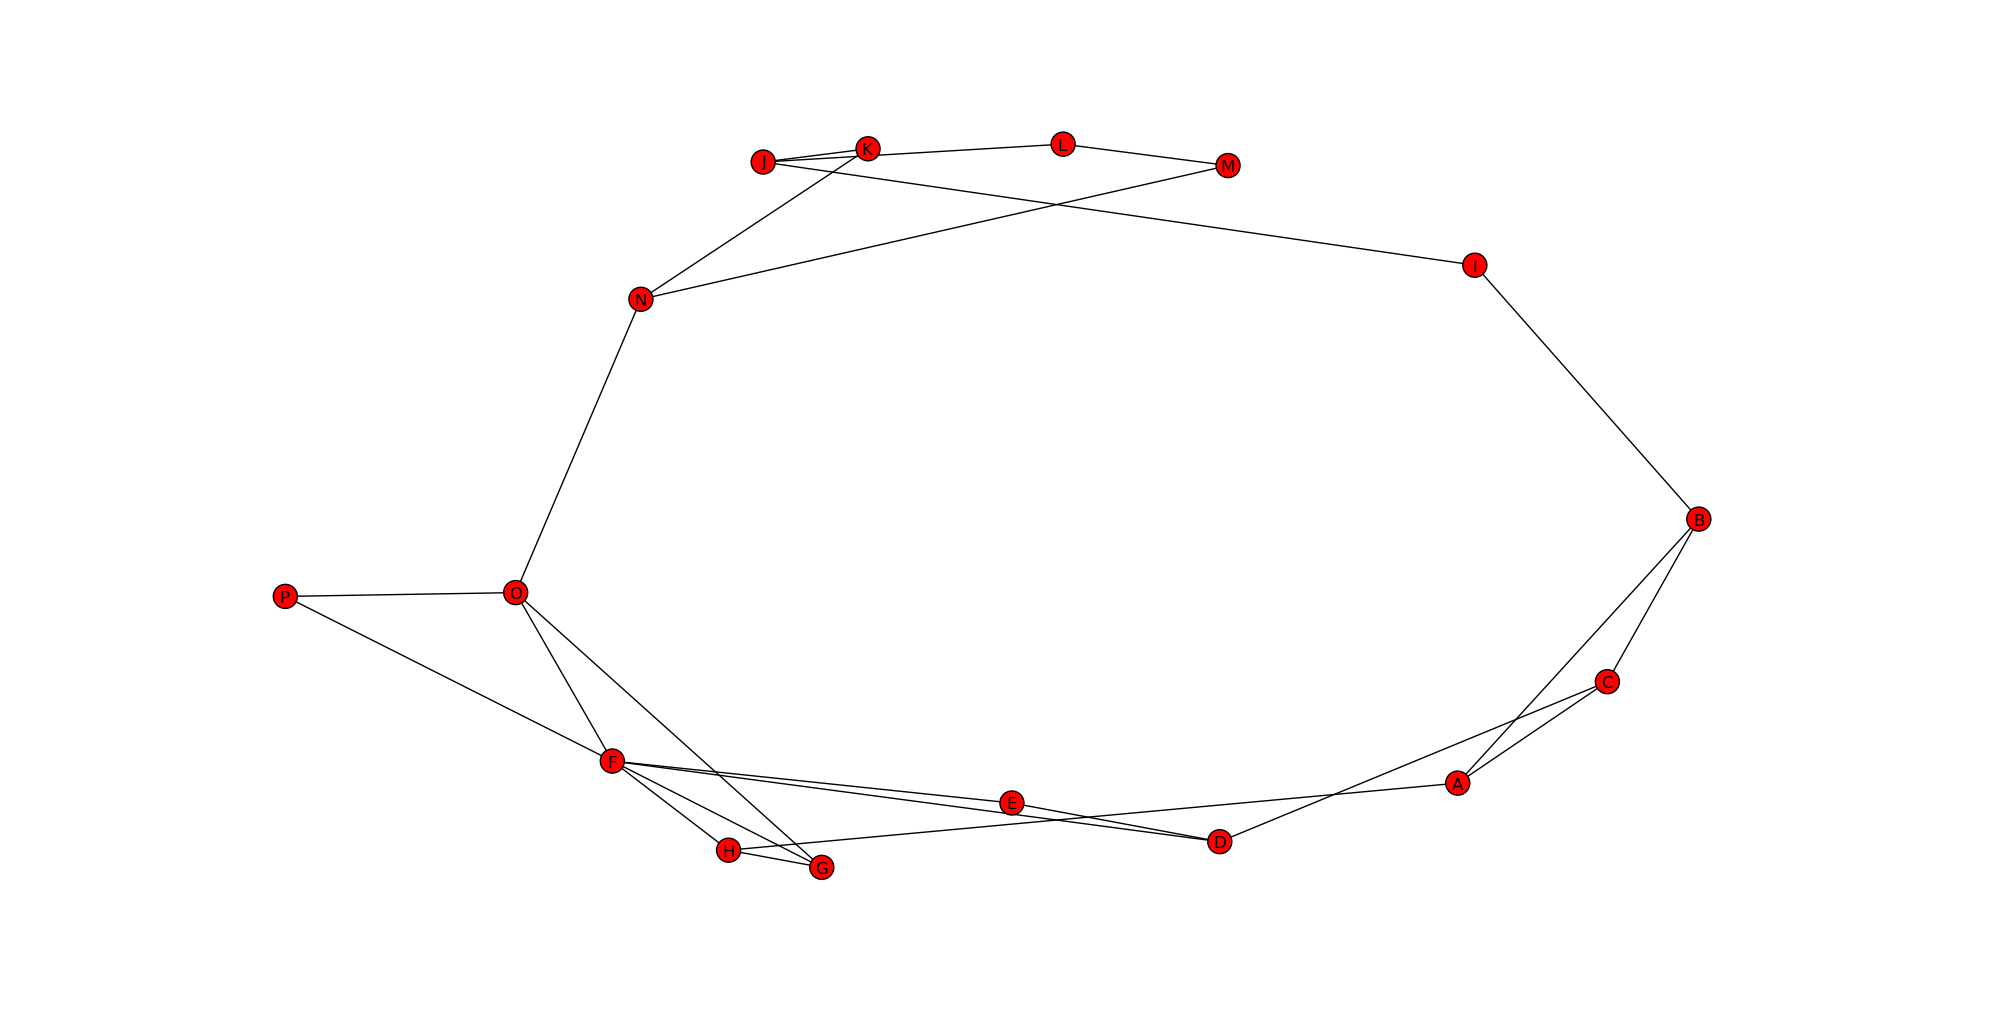
\includegraphics[width=0.75\columnwidth]{figure_1} % Example image
\end{center}
}
\subsection{Explanation}
Since all the links in the graph have the same cost in this algorithm, our implementation of always chose the first one in the list. Because of this, these links are quickly saturated which results in a large amount of blocked connections and a high amount of hops per circuit. A better way to implmement this algorithm would be to randomise the list of edges for each vertex before adding them to the open set, as this would allow more edges to be chosen and the connections to be better distributed. Vertex proximity does not ensure a lower propogation delay. As such, the average propogation delay under this algorithm is high. There are also many vertices in which the shortest path is through a single link. Using this algorithm quickly creates a bottleneck which results in many blocked connections. e.g. O - N, I - B.

The average degree of the topology is around 2. Because of this, you cant afford to only utilise 1 edge of the vertex. Because of this, Shortest Delay Path will block the most requests. It will always pick the edge with the shortest propogation delay. If both edges end up at a common vertex, the shortes propogation edge will saturated in a short amount of time and will let no more connections through. A side effect of this is that the connections that are let through will have the smallest total propogation delay possible. The smallest propogation delay does not ensure the least number of hops. If queueing + transmission + processing delay is significant, this is a very bad thing. Although this is a circuit network so its probably not that bad.

Least Loaded Path will get more valid paths as it actually considers how
loaded the paths are. Since this is the critereon by which paths are
rejected, the algorithm avoids paths which are already saturated. This ends up allowing much more through and distributes them
better. However, due to a wider distribution of connections, the connections
chosen may not be optimal. This results in a larger average propogation
delay than the other algorithms. It did result in a small number of hops per path as the paths were well distributed. This algorithm also avoids bottlenecks where the others do not.
\end{homeworkProblem}



%----------------------------------------------------------------------------------------

\end{document}
